\documentclass[aspectratio=169,11pt]{beamer}
\usetheme{Madrid}
\usecolortheme{seahorse}
\setbeamertemplate{navigation symbols}{}
\setbeamertemplate{headline}{}
\setbeamertemplate{footline}[frame number]
\setbeamertemplate{frametitle continuation}{}
\setbeamertemplate{frametitle}{\nointerlineskip\begin{beamercolorbox}[wd=\paperwidth,sep=0.45ex,leftskip=7.5mm,rightskip=7.5mm]{frametitle}\usebeamerfont{frametitle}\insertframetitle\end{beamercolorbox}}
\setbeamerfont{frametitle}{size=\large}
\setbeamerfont{normal text}{size=\normalsize}
\setbeamersize{text margin left=8mm,text margin right=8mm}
\setbeamercolor{keyphrase}{bg=blue!8,fg=black!85}
\setbeameroption{show notes}
\usepackage{pgfpages}
\pgfpagesuselayout{resize to}[a4paper,landscape]
\usepackage[T1]{fontenc}
\usepackage{tabularx}
\usepackage{array}
\usepackage{booktabs}
\usepackage{listings}
\usepackage{hyperref}
\usepackage{fancyvrb}
\lstdefinelanguage{mizar}{morekeywords={definition,end,struct,field,property,inherit,extends,where,from,let,be,being,mode,theorem,proof,thus,hence,by,registration,cluster,coherence,reduce,reducibility,import,for,holds,st,is,func,pred,attribute,algorithm,terminating,requires,ensures,do,while,invariant,decreasing,return,var,const,if,scheme,provided,environ,vocabularies,notations,constructors,registrations,theorems,begin,qua,reconsider,consider,such,that,not,or,and,implies,per,cases,set,thesis},sensitive=true,morecomment=[l]{::}}
\lstdefinelanguage{toml}{morecomment=[l]{\#},morestring=[b]"}
\lstset{basicstyle=\ttfamily\small,keywordstyle=\color{blue!50!black}\bfseries,commentstyle=\color{green!35!black}\itshape,stringstyle=\color{violet!70!black},showstringspaces=false,columns=fullflexible,keepspaces=true,backgroundcolor=\color{black!4},frame=single,rulecolor=\color{black!20},framesep=0.7mm,framerule=0.3pt,xleftmargin=1mm,xrightmargin=1mm,aboveskip=0.6mm,belowskip=0.8mm}
\newcommand{\statusbadge}[2]{\colorbox{#1}{\textcolor{white}{\strut\scriptsize\sffamily\bfseries #2}}}
\newcommand{\badgeMML}{\statusbadge{blue!45!black}{exact MML excerpt}}
\newcommand{\badgeSpec}{\statusbadge{green!35!black}{specification example}}
\newcommand{\badgeSketch}{\statusbadge{orange!75!black}{sketch}}
\newcommand{\deepdivetag}{\hfill\colorbox{black!15}{\textcolor{black!65}{\strut\scriptsize\sffamily deep dive}}}
\pdfstringdefDisableCommands{\def\translate#1{#1}}
\title{Mizar Evo: Design Principles}
\subtitle{Connecting automatic proof, readable mathematics, and checked computation\\ TPP 2026, RIKEN AIP Tokyo Office, November 2026\\ \textit{presenter notes edition}}
\author{Mizar Evo project}
\date{TPP 2026, RIKEN AIP Tokyo Office, November 16--17, 2026}

\begin{document}
\begin{frame}
\titlepage
\note{
\smallskip
\textbf{Read aloud:}
\begin{itemize}
\setlength{\itemsep}{1pt}
\setlength{\parsep}{0pt}
\setlength{\parskip}{0pt}
\item \textcolor{blue!55!black}{\textbf{Mizar is a proof checker. It has a fifty-year-old library, written in a readable mathematical language over first-order set theory.}}
\item \textcolor{blue!55!black}{\textbf{Mizar Evolution, or Mizar Evo, is a redesign of its language and tools. I will start with current Mizar's modernization challenges, then show how the new specification addresses them.}}
\item Everything I say has a label: fact, research hypothesis, or future direction.
\end{itemize}
}
\end{frame}

\section{Part 0. Introduction}
\begin{frame}[fragile,t]{0.2 - How To Read The Claims\deepdivetag}
\begin{footnotesize}
\setlength{\tabcolsep}{3pt}
\renewcommand{\arraystretch}{1.15}
\begin{tabularx}{\textwidth}{>{\raggedright\arraybackslash}X>{\raggedright\arraybackslash}X>{\raggedright\arraybackslash}X}
\toprule
\textbf{Level} & \textbf{Meaning} & \textbf{Marked how} \\
\midrule
fact & existing systems, published benchmarks, the Mizar Evo specification and main branch & no tag \\
research hypothesis & a claim that Mizar Evo is built to test & tagged in the text \\
future direction & a goal with no fixed date or design yet & tagged in the text \\
\bottomrule
\end{tabularx}
\end{footnotesize}

Code labels follow the Bialystok deck: exact MML excerpt, specification example, sketch.

\begin{itemize}
\setlength{\itemsep}{1pt}
\setlength{\parsep}{0pt}
\setlength{\parskip}{0pt}
\item The specification and the implementation are different things. One frame near the end separates them.
\end{itemize}
\note{
\smallskip
\textbf{Read aloud:}
\begin{itemize}
\setlength{\itemsep}{1pt}
\setlength{\parsep}{0pt}
\setlength{\parskip}{0pt}
\item Code labels follow the Bialystok deck: exact MML excerpt, specification example, sketch.
\item The specification and the implementation are different things. One frame near the end separates them.
\end{itemize}
}
\end{frame}

\begin{frame}[fragile,t]{0.3 - Current Mizar: Six Challenges And Design Principles}
\begin{footnotesize}
\setlength{\tabcolsep}{3pt}
\renewcommand{\arraystretch}{1.15}
\begin{tabularx}{\textwidth}{>{\raggedright\arraybackslash}X>{\raggedright\arraybackslash}X}
\toprule
\textbf{Challenge in modernizing Mizar} & \textbf{New design principle} \\
\midrule
\textcolor{blue!55!black}{\textbf{§1 Foundation:}} retain logic and MML; renew tools & First-order logic, set theory, and a small kernel \\
\textcolor{blue!55!black}{\textbf{§2 Writing:}} implicit types, registrations, overloads & Mathematical abstraction; explicit, traceable choices \\
\textcolor{blue!55!black}{\textbf{§3 Generics:}} separate definition and scheme mechanisms & Templates for definitions, theorems, and schemes \\
\textcolor{blue!55!black}{\textbf{§4 Computation:}} connect proofs and procedures & Contracts, invariants, and termination checks \\
\textcolor{blue!55!black}{\textbf{§5 Development:}} tools for a large library & Modules, namespaces, packages, incremental builds, LSP \\
\textcolor{blue!55!black}{\textbf{§6 Checking:}} external search and evidence & ATP flow; derive formula instances; trusted SAT check \\
\bottomrule
\end{tabularx}
\end{footnotesize}

\note{
Optional detail (see slide).

\smallskip
\textbf{Optional notes and sources:}
\begin{itemize}
\setlength{\itemsep}{1pt}
\setlength{\parsep}{0pt}
\setlength{\parskip}{0pt}
\item Each row pairs a challenge with its design principle. Sections 1–6 follow these rows. First-order logic and readable mathematics are assets to preserve.
\item The closing status frame separates the specification from implementation.
\item Source: specification 01, 18, 20, 21, 23; Bialystok problem-driven stories.
\end{itemize}
}
\end{frame}

\section{Part 1. Logical Foundation}
\begin{frame}[fragile,t]{1.1 - Keep The Foundation, Rebuild The Tools}
\begin{center}
\begin{beamercolorbox}[rounded=true,sep=2.5mm,wd=0.9\textwidth]{keyphrase}
\centering\itshape \textcolor{blue!55!black}{\textbf{Keep the mathematical layer.}}\\ \textcolor{blue!55!black}{\textbf{Rebuild the tools under it and around it.}}
\end{beamercolorbox}
\end{center}
\begin{itemize}
\setlength{\itemsep}{1pt}
\setlength{\parsep}{0pt}
\setlength{\parskip}{0pt}
\item \textcolor{blue!55!black}{\textbf{Mizar Evo keeps first-order logic and Tarski-Grothendieck set theory as the base logic.}}
\item It keeps soft types, modes, attributes, registrations, structures, and declarative proofs.
\item \textcolor{blue!55!black}{\textbf{Separate proof search from checking; a small kernel decides acceptance. Details in section 6.}}
\end{itemize}
\note{
\smallskip
\textbf{Read aloud:}
\begin{itemize}
\setlength{\itemsep}{1pt}
\setlength{\parsep}{0pt}
\setlength{\parskip}{0pt}
\item \textcolor{blue!55!black}{\textbf{Keep the mathematical layer.}} \textcolor{blue!55!black}{\textbf{Rebuild the tools under it and around it.}}
\item \textcolor{blue!55!black}{\textbf{Mizar Evo keeps first-order logic and Tarski-Grothendieck set theory as the base logic.}}
\item It keeps soft types, modes, attributes, registrations, structures, and declarative proofs.
\item \textcolor{blue!55!black}{\textbf{Separate proof search from checking; a small kernel decides acceptance. Details in section 6.}}
\end{itemize}
\smallskip
\textbf{Optional notes and sources:}
\begin{itemize}
\setlength{\itemsep}{1pt}
\setlength{\parsep}{0pt}
\setlength{\parskip}{0pt}
\item The shared structure concerns mathematical writing and proof tools, not identical logics or representations.
\item Neither success rates nor reconstruction failures show a first-order advantage. Evaluate ease of writing, automation, and proof checking.
\end{itemize}
}
\end{frame}

\begin{frame}[fragile,t]{1.2 - Current Mizar: Functions In Set Theory}
\smallskip
\textbf{Function application is a defined set-theoretic relation}~\badgeMML
\begin{lstlisting}[language={mizar},basicstyle=\ttfamily\small]
  func f.x -> set means
  :Def2:
  [x,it] in f if x in dom f otherwise it = {};
\end{lstlisting}
\smallskip
\textbf{A typed function is a soft type over partial functions}~\badgeMML
\begin{lstlisting}[language={mizar},basicstyle=\ttfamily\small]
definition
  let X,Y;
  mode Function of X,Y is quasi_total PartFunc of X,Y;
end;
\end{lstlisting}
\begin{itemize}
\setlength{\itemsep}{1pt}
\setlength{\parsep}{0pt}
\setlength{\parskip}{0pt}
\item \textcolor{blue!55!black}{\textbf{Here a function is an ordinary first-order object: a set of pairs. Application is defined, not built into the logic.}}
\item \textcolor{blue!55!black}{\textbf{Nothing in the base logic has to be higher-order.}}
\item The price: if you write raw set theory, the domain, the graph, functionality, and membership all appear in the text.
\end{itemize}
\note{
\smallskip
\textbf{Read aloud:}
\begin{itemize}
\setlength{\itemsep}{1pt}
\setlength{\parsep}{0pt}
\setlength{\parskip}{0pt}
\item Function application is a defined set-theoretic relation.
\item A typed function is a soft type over partial functions.
\item \textcolor{blue!55!black}{\textbf{Here a function is an ordinary first-order object: a set of pairs. Application is defined, not built into the logic.}}
\item \textcolor{blue!55!black}{\textbf{Nothing in the base logic has to be higher-order.}}
\item The price: if you write raw set theory, the domain, the graph, functionality, and membership all appear in the text.
\end{itemize}
\smallskip
\textbf{Optional notes and sources:}
\begin{itemize}
\setlength{\itemsep}{1pt}
\setlength{\parsep}{0pt}
\setlength{\parskip}{0pt}
\item Source: current MML \texttt{funct\_1.miz}, lines 138-140 (\texttt{FUNCT\_1:def 2}), and \texttt{funct\_2.miz}, lines 87-90 (checked October 7, 2026). URLs: \url{https://mizar.uwb.edu.pl/version/current/mml/funct\_1.miz}, \url{https://mizar.uwb.edu.pl/version/current/mml/funct\_2.miz}. GPL-3.0-or-later / CC-BY-SA-3.0-or-later.
\item \texttt{quasi\_total} (FUNCT\_2, lines 36-44) says the domain is all of X unless Y is empty.
\end{itemize}
}
\end{frame}

\section{Part 2. Readable Mathematics}
\begin{frame}[fragile,t]{2.1 - Preserve And Extend Mathematical Writing}
\smallskip
\textbf{What the author actually writes}~\badgeSketch~{\footnotesize(valid in current Mizar and Mizar Evo)}
\begin{lstlisting}[language={mizar},basicstyle=\ttfamily\small]
let X, Y be set;
let f be Function of X, Y;
let x be Element of X;
...  f.x  ...
\end{lstlisting}
\begin{itemize}
\setlength{\itemsep}{1pt}
\setlength{\parsep}{0pt}
\setlength{\parskip}{0pt}
\item \textcolor{blue!55!black}{\textbf{It is the same set-theoretic function. But the author writes \texttt{Function of X,Y} and \texttt{f.x}, not pairs and domains.}}
\item \textcolor{blue!55!black}{\textbf{Soft types, modes, attributes, registrations, schemes, and declarative proofs are not just a nicer way to write the same thing. They are the language design that lifts first-order set theory up to readable mathematics.}}
\item \textcolor{blue!55!black}{\textbf{New specification: preserve and extend mathematical writing; make implicit type, registration, and overload choices explicit and traceable.}}
\end{itemize}
\note{
\smallskip
\textbf{Read aloud:}
\begin{itemize}
\setlength{\itemsep}{1pt}
\setlength{\parsep}{0pt}
\setlength{\parskip}{0pt}
\item What the author actually writes.
\item \textcolor{blue!55!black}{\textbf{It is the same set-theoretic function. But the author writes \texttt{Function of X,Y} and \texttt{f.x}, not pairs and domains.}}
\item \textcolor{blue!55!black}{\textbf{Soft types, modes, attributes, registrations, schemes, and declarative proofs are not just a nicer way to write the same thing. They are the language design that lifts first-order set theory up to readable mathematics.}}
\item \textcolor{blue!55!black}{\textbf{New specification: preserve and extend mathematical writing; make implicit type, registration, and overload choices explicit and traceable.}}
\end{itemize}
}
\end{frame}

\begin{frame}[fragile,t]{2.2 - Make Operation Choices Explicit And Traceable}
\smallskip
\textbf{Select one of a ring's two operation views}~\badgeSketch
\begin{lstlisting}[language={mizar},basicstyle=\ttfamily\small]
let R be commutative Ring;
f(R);                  :: ambiguous Magma view
f(R qua AddMagma);      :: use addition
f(R qua MulMagma);      :: use multiplication
\end{lstlisting}
\begin{itemize}
\setlength{\itemsep}{1pt}
\setlength{\parsep}{0pt}
\setlength{\parskip}{0pt}
\item \textcolor{blue!55!black}{\textbf{Challenge: a ring has additive and multiplicative Magma views. \texttt{f(R)} is ambiguous.}}
\item \textcolor{blue!55!black}{\textbf{New specification: \texttt{qua} explicitly selects the additive or multiplicative view.}}
\item Trace automatically applied registrations and their derivation paths.
\end{itemize}
\note{
\smallskip
\textbf{Read aloud:}
\begin{itemize}
\setlength{\itemsep}{1pt}
\setlength{\parsep}{0pt}
\setlength{\parskip}{0pt}
\item Select one of a ring's two operation views.
\item \textcolor{blue!55!black}{\textbf{Challenge: a ring has additive and multiplicative Magma views. \texttt{f(R)} is ambiguous.}}
\item \textcolor{blue!55!black}{\textbf{New specification: \texttt{qua} explicitly selects the additive or multiplicative view.}}
\item Trace automatically applied registrations and their derivation paths.
\end{itemize}
\smallskip
\textbf{Optional notes and sources:}
\begin{itemize}
\setlength{\itemsep}{1pt}
\setlength{\parsep}{0pt}
\setlength{\parskip}{0pt}
\item f uses a Magma operation; definitions, inheritance, and registrations are assumed.
\item qua already exists in Mizar; this sketch illustrates explicit inheritance-path selection.
\item Source: \texttt{doc/spec/en/19.overload\_resolution.md} section 19.3.1; \texttt{17.clusters\_and\_registrations.md}, Traceability.
\end{itemize}
}
\end{frame}

\section{Part 3. Generic Mathematics}
\begin{frame}[fragile,t]{3.1 - Templates: Share Functor Definitions And Result Types}
\textcolor{blue!55!black}{\textbf{Example: the sum of functions. Add their values at each point.}}

\smallskip
\textbf{Generic functor}~\badgeSketch~{\footnotesize(existence and uniqueness proofs omitted)}
\begin{lstlisting}[language={mizar},basicstyle=\ttfamily\small]
definition
  let T be type extends non empty AddMagma;
  let I be non empty set;
  let f, g be Function of I, T;
  func AddDef: Add[T,I](f,g) -> Function of I,T means
    for i being Element of I holds it.i = T.add(f.i,g.i);
end;
\end{lstlisting}
\begin{itemize}
\setlength{\itemsep}{1pt}
\setlength{\parsep}{0pt}
\setlength{\parskip}{0pt}
\item \textcolor{blue!55!black}{\textbf{Current MML: real and complex result types need separate redefinitions and registrations.}}
\item \textcolor{blue!55!black}{\textbf{New specification: parameterize the value type T to share the definition and result type.}}
\end{itemize}
\note{
\smallskip
\textbf{Read aloud:}
\begin{itemize}
\setlength{\itemsep}{1pt}
\setlength{\parsep}{0pt}
\setlength{\parskip}{0pt}
\item \textcolor{blue!55!black}{\textbf{Example: the sum of functions. Add their values at each point.}}
\item Generic functor.
\item \textcolor{blue!55!black}{\textbf{Current MML: real and complex result types need separate redefinitions and registrations.}}
\item \textcolor{blue!55!black}{\textbf{New specification: parameterize the value type T to share the definition and result type.}}
\end{itemize}
\smallskip
\textbf{Optional notes and sources:}
\begin{itemize}
\setlength{\itemsep}{1pt}
\setlength{\parsep}{0pt}
\setlength{\parskip}{0pt}
\item T supplies addition; I is a common nonempty domain. Suitable structures and registrations are assumed.
\item Source: \texttt{doc/spec/en/18.templates.md} sections 18.2.2, 18.7, 18.10.1; \texttt{sample\_codes.md} AddMagma; MML VALUED\_1 (\url{https://mizar.uwb.edu.pl/version/current/html/valued\_1.html}).
\end{itemize}
}
\end{frame}

\begin{frame}[fragile,t]{3.2 - Schemes Become Ordinary Templates\deepdivetag}
\smallskip
\textbf{Induction as a theorem with a predicate parameter}~\badgeSpec
\begin{lstlisting}[language={mizar},basicstyle=\ttfamily\small]
definition
  let P be pred(Nat);
  theorem NatInduction[P]:
    P(0) & (for n being Nat st P(n) holds P(n+1))
    implies for n being Nat holds P(n)
  proof ... end;
end;
\end{lstlisting}
\begin{itemize}
\setlength{\itemsep}{1pt}
\setlength{\parsep}{0pt}
\setlength{\parskip}{0pt}
\item A predicate parameter gives a family of first-order theorems, one for each predicate you put in.
\item Instantiation is explicit: \texttt{by NatInduction[P], Base, Step} after a \texttt{defpred}.
\item Functor parameters are schema-level symbols, not sets. This keeps the logic first-order.
\item Details: Bialystok deck, Story 6 (\texttt{PermProduct[T]}, \texttt{qua} views), and Backup 4 here.
\end{itemize}
\note{
\smallskip
\textbf{Read aloud:}
\begin{itemize}
\setlength{\itemsep}{1pt}
\setlength{\parsep}{0pt}
\setlength{\parskip}{0pt}
\item Induction as a theorem with a predicate parameter.
\item A predicate parameter gives a family of first-order theorems, one for each predicate you put in.
\item Instantiation is explicit: \texttt{by NatInduction[P], Base, Step} after a \texttt{defpred}.
\item Functor parameters are schema-level symbols, not sets. This keeps the logic first-order.
\item Details: Bialystok deck, Story 6 (\texttt{PermProduct[T]}, \texttt{qua} views), and Backup 4 here.
\end{itemize}
}
\end{frame}

\section{Part 4. Verified Computation}
\begin{frame}[fragile,t]{4.1 - Computation: Verified Algorithms}
\begin{itemize}
\setlength{\itemsep}{1pt}
\setlength{\parsep}{0pt}
\setlength{\parskip}{0pt}
\item Mizar uses declarative proofs and built-in automation. It has no user-programmable tactic language.
\item \textcolor{blue!55!black}{\textbf{Challenge: connect mathematical proofs and executable computation in one checking framework.}}
\item \textcolor{blue!55!black}{\textbf{New specification: an algorithm is a procedure with a contract. Its correctness, invariants, and termination are checked.}}
\item Uses: verify algorithms themselves, and use verified procedures to support proofs.
\end{itemize}
\note{
\smallskip
\textbf{Read aloud:}
\begin{itemize}
\setlength{\itemsep}{1pt}
\setlength{\parsep}{0pt}
\setlength{\parskip}{0pt}
\item Mizar uses declarative proofs and built-in automation. It has no user-programmable tactic language.
\item \textcolor{blue!55!black}{\textbf{Challenge: connect mathematical proofs and executable computation in one checking framework.}}
\item \textcolor{blue!55!black}{\textbf{New specification: an algorithm is a procedure with a contract. Its correctness, invariants, and termination are checked.}}
\item Uses: verify algorithms themselves, and use verified procedures to support proofs.
\end{itemize}
\smallskip
\textbf{Optional notes and sources:}
\begin{itemize}
\setlength{\itemsep}{1pt}
\setlength{\parsep}{0pt}
\setlength{\parskip}{0pt}
\item Source: \texttt{doc/spec/en/20.algorithm\_and\_verification.md}, sections 20.1 and 20.12.
\end{itemize}
}
\end{frame}

\begin{frame}[fragile,t]{4.2 - Algorithms: Contracts, Proofs, Computation}
\smallskip
\textbf{\textcolor{blue!55!black}{\textbf{Euclid's algorithm with a contract}}}~\badgeSpec
\begin{lstlisting}[language={mizar},basicstyle=\ttfamily\footnotesize]
terminating algorithm euclid_gcd(a, b) -> Nat
  requires a >= 1 & b >= 1
  ensures result = Gcd(a, b)
do
  var x := a;  var y := b;
  while y <> 0 do
    invariant x >= 1 & y >= 0 & Gcd(a, b) = Gcd(x, y);  decreasing y;
    const r := x mod y;  x := y;  y := r;
  end;
  return x;
end;
\end{lstlisting}
\begin{itemize}
\setlength{\itemsep}{1pt}
\setlength{\parsep}{0pt}
\setlength{\parskip}{0pt}
\item \textcolor{blue!55!black}{\textbf{Contracts, invariants, and termination measures become first-order proof obligations, checked like theorems.}}
\item \textcolor{blue!55!black}{\textbf{Two roles: a verified automation procedure, and a checked computation run by \texttt{by computation}. Status: specified. MVM execution and code extraction come later.}}
\end{itemize}
\note{
\smallskip
\textbf{Read aloud:}
\begin{itemize}
\setlength{\itemsep}{1pt}
\setlength{\parsep}{0pt}
\setlength{\parskip}{0pt}
\item \textcolor{blue!55!black}{\textbf{Euclid's algorithm with a contract}}.
\item \textcolor{blue!55!black}{\textbf{Contracts, invariants, and termination measures become first-order proof obligations, checked like theorems.}}
\item \textcolor{blue!55!black}{\textbf{Two roles: a verified automation procedure, and a checked computation run by \texttt{by computation}. Status: specified. MVM execution and code extraction come later.}}
\end{itemize}
\smallskip
\textbf{Optional notes and sources:}
\begin{itemize}
\setlength{\itemsep}{1pt}
\setlength{\parsep}{0pt}
\setlength{\parskip}{0pt}
\item Source: \texttt{doc/spec/en/20.algorithm\_and\_verification.md}, section 20.12 (condensed: the enclosing \texttt{definition} block and \texttt{let a, b be Nat;} are omitted).
\end{itemize}
}
\end{frame}

\begin{frame}[fragile,t]{4.3 - Future Targets For Algorithms\deepdivetag}
\smallskip
\textbf{Future direction, not current capability:}
\begin{itemize}
\setlength{\itemsep}{1pt}
\setlength{\parsep}{0pt}
\setlength{\parskip}{0pt}
\item number-theoretic and combinatorial algorithms; symbolic algorithms; optimization procedures;
\item later: cryptographic algorithms and protocols; quantum and hybrid classical-quantum algorithms.
\end{itemize}
\smallskip
\textbf{One workflow for all of them:}
\begin{enumerate}
\setlength{\itemsep}{1pt}
\setlength{\parsep}{0pt}
\setlength{\parskip}{0pt}
\item write the procedure; 2. state the contract; 3. give invariants and termination; 4. generate proof obligations; 5. prove them with ATPs and check them in the kernel; 6. run on concrete inputs; 7. extract code later.
\end{enumerate}
\begin{itemize}
\setlength{\itemsep}{1pt}
\setlength{\parsep}{0pt}
\setlength{\parskip}{0pt}
\item \textcolor{blue!55!black}{\textbf{Algorithms make the gap between tactics and application algorithms smaller. The targets above are future directions.}}
\end{itemize}
\note{
\smallskip
\textbf{Read aloud:}
\begin{itemize}
\setlength{\itemsep}{1pt}
\setlength{\parsep}{0pt}
\setlength{\parskip}{0pt}
\item number-theoretic and combinatorial algorithms; symbolic algorithms; optimization procedures;
\item later: cryptographic algorithms and protocols; quantum and hybrid classical-quantum algorithms.
\item write the procedure; 2. state the contract; 3. give invariants and termination; 4. generate proof obligations; 5. prove them with ATPs and check them in the kernel; 6. run on concrete inputs; 7. extract code later.
\item \textcolor{blue!55!black}{\textbf{Algorithms make the gap between tactics and application algorithms smaller. The targets above are future directions.}}
\end{itemize}
}
\end{frame}

\section{Part 5. Development Infrastructure}
\begin{frame}[fragile,t]{5.1 - Development Problems And The New Design}
\begin{footnotesize}
\setlength{\tabcolsep}{3pt}
\renewcommand{\arraystretch}{1.15}
\begin{tabularx}{\textwidth}{>{\raggedright\arraybackslash}X>{\raggedright\arraybackslash}X}
\toprule
\textbf{Seen after fifty years of MML} & \textbf{Mizar Evo} \\
\midrule
the article as the unit of dependency & modules with explicit imports \\
global name management & namespaces, fully qualified names \\
weak distribution and versioning & packages, SemVer, lock files \\
full rebuilds & incremental builds with dependency fingerprints \\
ATP as an add-on, automation hard to see & first-class ATP pipeline, resolution traces, kernel evidence \\
weak IDE and machine-readable I/O & LSP, structured diagnostics, agent interface \\
\bottomrule
\end{tabularx}
\end{footnotesize}

\begin{itemize}
\setlength{\itemsep}{1pt}
\setlength{\parsep}{0pt}
\setlength{\parskip}{0pt}
\item \textcolor{blue!55!black}{\textbf{Keeping Mizar's mathematical ideas and keeping 1970s software architecture are two different things.}}
\item \textcolor{blue!55!black}{\textbf{Of course, we also modernize the whole development infrastructure. The Bialystok deck has the details. Here one table is enough.}}
\end{itemize}
\note{
\smallskip
\textbf{Read aloud:}
\begin{itemize}
\setlength{\itemsep}{1pt}
\setlength{\parsep}{0pt}
\setlength{\parskip}{0pt}
\item \textcolor{blue!55!black}{\textbf{Keeping Mizar's mathematical ideas and keeping 1970s software architecture are two different things.}}
\item \textcolor{blue!55!black}{\textbf{Of course, we also modernize the whole development infrastructure. The Bialystok deck has the details. Here one table is enough.}}
\end{itemize}
\smallskip
\textbf{Optional notes and sources:}
\begin{itemize}
\setlength{\itemsep}{1pt}
\setlength{\parsep}{0pt}
\setlength{\parskip}{0pt}
\item This is not a criticism. It is software engineering that was not common fifty years ago, brought into a formal mathematics environment.
\item Details: Bialystok deck, Stories 1, 3, 5, 8; Backups 6-8 here.
\end{itemize}
}
\end{frame}

\begin{frame}[fragile,t]{5.2 - The Whole Picture}
\begin{center}
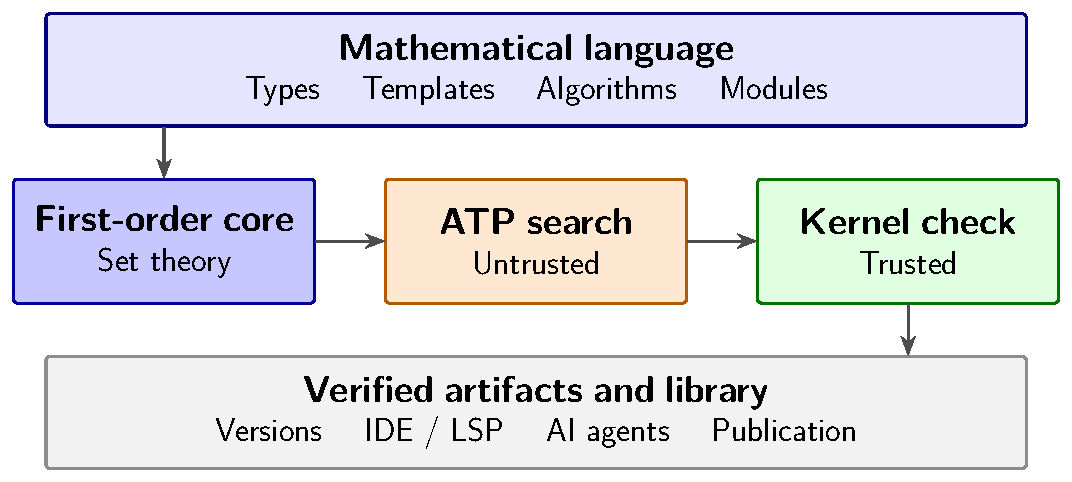
\includegraphics[width=\textwidth,height=0.64\textheight,keepaspectratio]{figures/layer_stack.pdf}
\end{center}
\begin{itemize}
\setlength{\itemsep}{1pt}
\setlength{\parsep}{0pt}
\setlength{\parskip}{0pt}
\item \textcolor{blue!55!black}{\textbf{Rich mathematics, a small first-order core, and modern infrastructure.}}
\end{itemize}
\note{
\smallskip
\textbf{Read aloud:}
\begin{itemize}
\setlength{\itemsep}{1pt}
\setlength{\parsep}{0pt}
\setlength{\parskip}{0pt}
\item \textcolor{blue!55!black}{\textbf{Rich mathematics, a small first-order core, and modern infrastructure.}}
\end{itemize}
\smallskip
\textbf{Optional notes and sources:}
\begin{itemize}
\setlength{\itemsep}{1pt}
\setlength{\parsep}{0pt}
\setlength{\parskip}{0pt}
\item Elaboration maps the mathematical language to a first-order representation. The kernel checks evidence proposed by external ATPs. Verified artifacts and the library support IDE / LSP, AI, and publication.
\end{itemize}
}
\end{frame}

\section{Part 6. Checking And Automation}
\begin{frame}[fragile,t]{6.1 - Automation: Separate Search From Checking}
\begin{center}
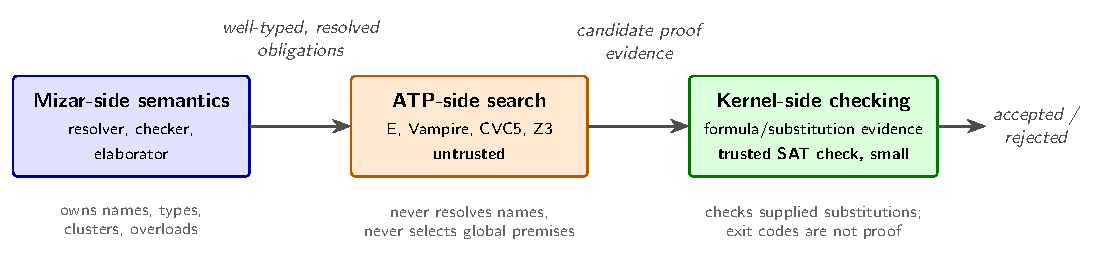
\includegraphics[width=\textwidth,height=0.52\textheight,keepaspectratio]{../2026-09-bialystok/figures/reasoning_boundary.pdf}
\end{center}
\begin{itemize}
\setlength{\itemsep}{1pt}
\setlength{\parsep}{0pt}
\setlength{\parskip}{0pt}
\item \textcolor{blue!55!black}{\textbf{A first-order ATP is a powerful searcher. It is not a trusted checker.}}
\item \textcolor{blue!55!black}{\textbf{The Mizar side owns names, types, clusters, and overloads. Provers own search. The kernel owns acceptance: it checks the given formulas and substitutions with a small, trusted SAT check.}}
\item A prover's exit code is never a proof. This is how first-order automation can be a design principle without making the trusted base bigger.
\end{itemize}
\note{
\smallskip
\textbf{Read aloud:}
\begin{itemize}
\setlength{\itemsep}{1pt}
\setlength{\parsep}{0pt}
\setlength{\parskip}{0pt}
\item \textcolor{blue!55!black}{\textbf{A first-order ATP is a powerful searcher. It is not a trusted checker.}}
\item \textcolor{blue!55!black}{\textbf{The Mizar side owns names, types, clusters, and overloads. Provers own search. The kernel owns acceptance: it checks the given formulas and substitutions with a small, trusted SAT check.}}
\item A prover's exit code is never a proof. This is how first-order automation can be a design principle without making the trusted base bigger.
\end{itemize}
\smallskip
\textbf{Optional notes and sources:}
\begin{itemize}
\setlength{\itemsep}{1pt}
\setlength{\parsep}{0pt}
\setlength{\parskip}{0pt}
\item Source: \texttt{doc/design/architecture/en/08.reasoning\_boundary.md}; Bialystok deck, Story 4; Backup 5 here shows what the evidence contains.
\end{itemize}
}
\end{frame}

\begin{frame}[fragile,t]{6.2 - Using ATPs: Search, Check, And Reuse}
\begin{center}
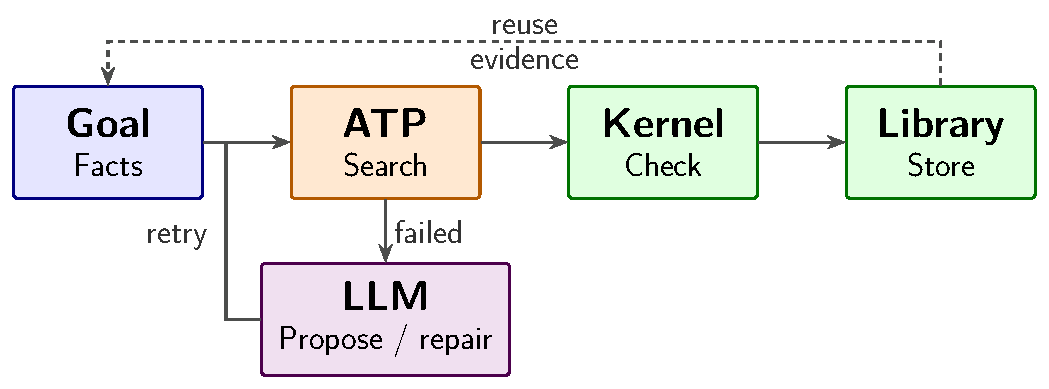
\includegraphics[width=\textwidth,height=0.54\textheight,keepaspectratio]{figures/llm_atp_loop.pdf}
\end{center}
\begin{itemize}
\setlength{\itemsep}{1pt}
\setlength{\parsep}{0pt}
\setlength{\parskip}{0pt}
\item \textcolor{blue!55!black}{\textbf{Goal and facts → ATP search → kernel check → store in the library and reuse.}}
\item For open goals, revise lemmas or the plan and retry. The figure shows design intent.
\end{itemize}
\note{
\smallskip
\textbf{Read aloud:}
\begin{itemize}
\setlength{\itemsep}{1pt}
\setlength{\parsep}{0pt}
\setlength{\parskip}{0pt}
\item \textcolor{blue!55!black}{\textbf{Goal and facts → ATP search → kernel check → store in the library and reuse.}}
\item For open goals, revise lemmas or the plan and retry. The figure shows design intent.
\end{itemize}
\smallskip
\textbf{Optional notes and sources:}
\begin{itemize}
\setlength{\itemsep}{1pt}
\setlength{\parsep}{0pt}
\setlength{\parskip}{0pt}
\item LLMs can help propose and repair. Acceptance depends on the evidence check, explained on the next frame.
\item Current ATP input is cited premises and local hypotheses. Whole-library premise selection and the loop's cost-effectiveness remain evaluation targets.
\item Source: \texttt{doc/spec/en/21.source\_code\_annotation\_and\_atp.md} section 21.7.2; \texttt{doc/design/architecture/en/21.ai\_agent\_interface.md}.
\end{itemize}
}
\end{frame}

\begin{frame}[fragile,t]{6.3 - From Evidence To Instances To SAT Checking}
\begin{center}
\begin{beamercolorbox}[rounded=true,sep=2.5mm,wd=0.9\textwidth]{keyphrase}
\centering\itshape \textcolor{blue!55!black}{\textbf{Evidence → Formula instances → SAT check}}
\end{beamercolorbox}
\end{center}
\begin{enumerate}
\setlength{\itemsep}{1pt}
\setlength{\parsep}{0pt}
\setlength{\parskip}{0pt}
\item \textcolor{blue!55!black}{\textbf{Evidence:}} source formulas, explicit substitutions, provenance, and the target goal.
\item \textcolor{blue!55!black}{\textbf{Kernel:}} check the bindings and substitutions, then derive the formula instances.
\item \textcolor{blue!55!black}{\textbf{SAT:}} encode the instances and the negated goal. Accept only after the trusted checker confirms UNSAT.
\end{enumerate}
\note{
\smallskip
\textbf{Read aloud:}
\begin{itemize}
\setlength{\itemsep}{1pt}
\setlength{\parsep}{0pt}
\setlength{\parskip}{0pt}
\item \textcolor{blue!55!black}{\textbf{Evidence → Formula instances → SAT check}}
\item \textcolor{blue!55!black}{\textbf{Evidence:}} source formulas, explicit substitutions, provenance, and the target goal.
\item \textcolor{blue!55!black}{\textbf{Kernel:}} check the bindings and substitutions, then derive the formula instances.
\item \textcolor{blue!55!black}{\textbf{SAT:}} encode the instances and the negated goal. Accept only after the trusted checker confirms UNSAT.
\end{itemize}
\smallskip
\textbf{Optional notes and sources:}
\begin{itemize}
\setlength{\itemsep}{1pt}
\setlength{\parsep}{0pt}
\setlength{\parskip}{0pt}
\item UNSAT establishes the goal from the premises. The kernel derives the instances and SAT problem itself.
\item Backend traces and exit codes are diagnostic only. Full evidence fields: Backup 5.
\item Source: \texttt{doc/design/architecture/en/08.reasoning\_boundary.md}, \texttt{15.kernel\_certificate\_format.md}.
\end{itemize}
}
\end{frame}

\section{Status And Roadmap}
\begin{frame}[fragile,t]{Where The Project Stands (October 2026)}
\begin{itemize}
\setlength{\itemsep}{1pt}
\setlength{\parsep}{0pt}
\setlength{\parskip}{0pt}
\item \textcolor{blue!55!black}{\textbf{Specification: 24 chapters plus appendices. English is the canonical language.}}
\item \textcolor{blue!55!black}{\textbf{Implemented on the main branch: the Rust frontend (lexer, parser, syntax tree); name resolution and type checking on an alpha corpus; proof-obligation generation with deterministic discharge; ATP problem encoding and candidate evidence; SAT-backed kernel evidence checking; cache, fingerprint, and build-scheduling milestones.}}
\item \textcolor{blue!55!black}{\textbf{In progress: end-to-end integration from source to verified artifact; the LSP server; the documentation generator.}}
\item \textcolor{blue!55!black}{\textbf{Planned for later: MVM execution, code extraction, library-wide premise selection, MML migration.}}
\item This talk does not claim any end-to-end results with external provers.
\end{itemize}
\note{
\smallskip
\textbf{Read aloud:}
\begin{itemize}
\setlength{\itemsep}{1pt}
\setlength{\parsep}{0pt}
\setlength{\parskip}{0pt}
\item \textcolor{blue!55!black}{\textbf{Specification: 24 chapters plus appendices. English is the canonical language.}}
\item \textcolor{blue!55!black}{\textbf{Implemented on the main branch: the Rust frontend (lexer, parser, syntax tree); name resolution and type checking on an alpha corpus; proof-obligation generation with deterministic discharge; ATP problem encoding and candidate evidence; SAT-backed kernel evidence checking; cache, fingerprint, and build-scheduling milestones.}}
\item \textcolor{blue!55!black}{\textbf{In progress: end-to-end integration from source to verified artifact; the LSP server; the documentation generator.}}
\item \textcolor{blue!55!black}{\textbf{Planned for later: MVM execution, code extraction, library-wide premise selection, MML migration.}}
\item This talk does not claim any end-to-end results with external provers.
\end{itemize}
\smallskip
\textbf{Optional notes and sources:}
\begin{itemize}
\setlength{\itemsep}{1pt}
\setlength{\parsep}{0pt}
\setlength{\parskip}{0pt}
\item Source: \texttt{doc/design/todo.md}, Crate Status, as of October 7, 2026. Re-check before the talk.
\end{itemize}
}
\end{frame}

\begin{frame}[fragile,t]{Roadmap}
\begin{center}
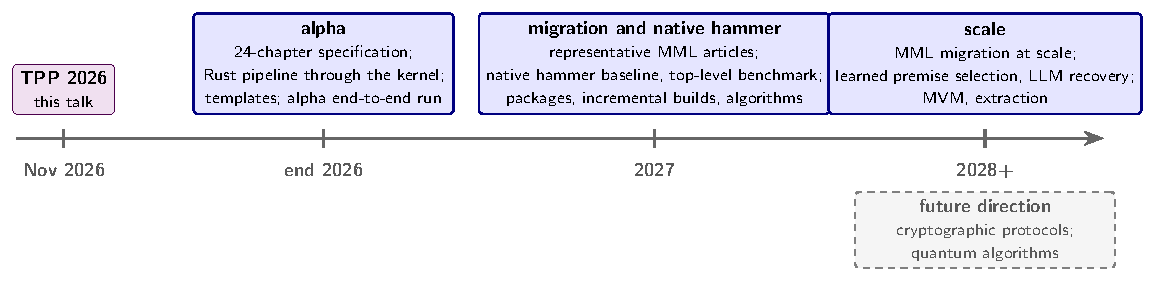
\includegraphics[width=\textwidth,height=0.46\textheight,keepaspectratio]{figures/roadmap_tpp.pdf}
\end{center}
\begin{itemize}
\setlength{\itemsep}{1pt}
\setlength{\parsep}{0pt}
\setlength{\parskip}{0pt}
\item \textcolor{blue!55!black}{\textbf{2026: finish the specification, the Rust pipeline through the kernel, template processing, and an alpha end-to-end run.}}
\item \textcolor{blue!55!black}{\textbf{2027: migrate representative MML articles, build a native hammer baseline, and benchmark on top-level theorems, in the same units MizAR uses.}}
\item 2028 and later: scale up the migration; learned premise selection; LLM-assisted failure recovery; MVM and extraction. Cryptographic and quantum targets stay future directions.
\end{itemize}
\note{
\smallskip
\textbf{Read aloud:}
\begin{itemize}
\setlength{\itemsep}{1pt}
\setlength{\parsep}{0pt}
\setlength{\parskip}{0pt}
\item \textcolor{blue!55!black}{\textbf{2026: finish the specification, the Rust pipeline through the kernel, template processing, and an alpha end-to-end run.}}
\item \textcolor{blue!55!black}{\textbf{2027: migrate representative MML articles, build a native hammer baseline, and benchmark on top-level theorems, in the same units MizAR uses.}}
\item 2028 and later: scale up the migration; learned premise selection; LLM-assisted failure recovery; MVM and extraction. Cryptographic and quantum targets stay future directions.
\end{itemize}
}
\end{frame}

\begin{frame}[fragile,t]{Closing}
\begin{center}
\begin{beamercolorbox}[rounded=true,sep=2.5mm,wd=0.9\textwidth]{keyphrase}
\centering\itshape \textcolor{blue!55!black}{\textbf{Keep the foundation small.}}\\ \textcolor{blue!55!black}{\textbf{Keep the mathematics readable.}}\\ \textcolor{blue!55!black}{\textbf{Modernize everything else.}}
\end{beamercolorbox}
\end{center}
\begin{itemize}
\setlength{\itemsep}{1pt}
\setlength{\parsep}{0pt}
\setlength{\parskip}{0pt}
\item \textcolor{blue!55!black}{\textbf{Thank you. I welcome your questions, especially on MML migration, usability, and how to evaluate automation.}}
\end{itemize}
\note{
\smallskip
\textbf{Read aloud:}
\begin{itemize}
\setlength{\itemsep}{1pt}
\setlength{\parsep}{0pt}
\setlength{\parskip}{0pt}
\item \textcolor{blue!55!black}{\textbf{Keep the foundation small.}} \textcolor{blue!55!black}{\textbf{Keep the mathematics readable.}} \textcolor{blue!55!black}{\textbf{Modernize everything else.}}
\item \textcolor{blue!55!black}{\textbf{Thank you. I welcome your questions, especially on MML migration, usability, and how to evaluate automation.}}
\end{itemize}
}
\end{frame}

\appendix
\section{Backup 1. MizAR 60 In Detail}
\begin{frame}[fragile,t]{Backup 1. MizAR 60 In Detail}
Source: Jakubův et al., MizAR 60 for Mizar 50, ITP 2023.

\begin{itemize}
\setlength{\itemsep}{1pt}
\setlength{\parsep}{0pt}
\setlength{\parskip}{0pt}
\item Dataset: MML 1147 exported by MPTP, 57,897 theorems including unnamed top-level lemmas; the same version as the MizAR 40 evaluation, so the results can be compared.
\item Holdout: 1,690 / 2,896 (58.4\%), without user premise help, 420 CPU s. Training/development/holdout: 90:5:5 (MizAR 40: about 40.6\%).
\item Over 75\% proved when the premises can be chosen from the library by a human or a machine (MizAR 40: 56\%).
\item Strongest single method: 40\% in 30 s in hammering mode; 60\% in 120 s with human premises.
\item Transfer: the strongest method also works on 13,370 new theorems from 242 new articles in MML 1382.
\item Methods: E and Vampire with ENIGMA and Deepire guidance, learned premise selection, and a loop that trains on millions of ATP proofs.
\end{itemize}
\note{
\smallskip
\textbf{Read aloud:}
\begin{itemize}
\setlength{\itemsep}{1pt}
\setlength{\parsep}{0pt}
\setlength{\parskip}{0pt}
\item Dataset: MML 1147 exported by MPTP, 57,897 theorems including unnamed top-level lemmas; the same version as the MizAR 40 evaluation, so the results can be compared.
\item Holdout: 1,690 / 2,896 (58.4\%), without user premise help, 420 CPU s. Training/development/holdout: 90:5:5 (MizAR 40: about 40.6\%).
\item Over 75\% proved when the premises can be chosen from the library by a human or a machine (MizAR 40: 56\%).
\item Strongest single method: 40\% in 30 s in hammering mode; 60\% in 120 s with human premises.
\item Transfer: the strongest method also works on 13,370 new theorems from 242 new articles in MML 1382.
\item Methods: E and Vampire with ENIGMA and Deepire guidance, learned premise selection, and a loop that trains on millions of ATP proofs.
\end{itemize}
\smallskip
\textbf{Optional notes and sources:}
\begin{itemize}
\setlength{\itemsep}{1pt}
\setlength{\parsep}{0pt}
\setlength{\parskip}{0pt}
\item Source: Jakubův et al., MizAR 60 for Mizar 50, ITP 2023.
\end{itemize}
}
\end{frame}

\section{Backup 2. Sledgehammer Evaluations In Detail}
\begin{frame}[fragile,t]{Backup 2. Sledgehammer Evaluations In Detail}
\begin{footnotesize}
\setlength{\tabcolsep}{3pt}
\renewcommand{\arraystretch}{1.15}
\begin{tabularx}{\textwidth}{>{\raggedright\arraybackslash}X>{\raggedright\arraybackslash}X>{\raggedright\arraybackslash}X}
\toprule
\textbf{Evaluation} & \textbf{Dataset and method} & \textbf{Success} \\
\midrule
ITP 2022 & 5,000 AFP goals, 16 greedy configurations & 68.8\% \\
Magnushammer (preprint 2023) & 1,000 PISA theorems, Sledgehammer & 38.3\% \\
Same PISA evaluation & Magnushammer with learned premise selection & 59.5\% \\
\bottomrule
\end{tabularx}
\end{footnotesize}

\begin{itemize}
\setlength{\itemsep}{1pt}
\setlength{\parsep}{0pt}
\setlength{\parskip}{0pt}
\item ITP 2022: 50 entries, 100 goals each; MePo, 512 facts in the base setting, 30 CPU seconds per configuration. Configurations are selected using the evaluation set. Reconstruction is not evaluated.
\item PISA: Isabelle2021-1, Sledgehammer timeout 30 seconds, five local provers, union over several settings. Success requires a proof checked by Isabelle.
\item Close dates do not make local goals and whole theorems, or search success and checked proofs, the same measure.
\end{itemize}
\note{
\smallskip
\textbf{Read aloud:}
\begin{itemize}
\setlength{\itemsep}{1pt}
\setlength{\parsep}{0pt}
\setlength{\parskip}{0pt}
\item ITP 2022: 50 entries, 100 goals each; MePo, 512 facts in the base setting, 30 CPU seconds per configuration. Configurations are selected using the evaluation set. Reconstruction is not evaluated.
\item PISA: Isabelle2021-1, Sledgehammer timeout 30 seconds, five local provers, union over several settings. Success requires a proof checked by Isabelle.
\item Close dates do not make local goals and whole theorems, or search success and checked proofs, the same measure.
\end{itemize}
\smallskip
\textbf{Optional notes and sources:}
\begin{itemize}
\setlength{\itemsep}{1pt}
\setlength{\parsep}{0pt}
\setlength{\parskip}{0pt}
\item Source: Desharnais et al., Seventeen Provers Under the Hammer, ITP 2022, sections 5, 5.6, Table 10; Miku\l{}a et al., Magnushammer, arXiv:2303.04488 (preprint 2023), Table 2, Appendix A.4.
\end{itemize}
}
\end{frame}

\section{Backup 3. HOL-To-FOL Encodings And Reconstruction}
\begin{frame}[fragile,t]{Backup 3. HOL-To-FOL Encodings And Reconstruction}
\begin{itemize}
\setlength{\itemsep}{1pt}
\setlength{\parsep}{0pt}
\setlength{\parskip}{0pt}
\item Function application: a variable function applied to an argument becomes \texttt{app(F, X)}; applications of constants may stay curried or be flattened.
\item Lambda abstraction: lambda lifting introduces fresh constants with defining equations; combinator translation is the alternative.
\item Types: polymorphic HOL types are encoded by guards, tags, or monomorphization; the choice affects soundness, completeness, and prover performance.
\item Booleans: Boolean-valued terms inside formulas need a separate encoding.
\item Reconstruction: \texttt{metis} with the used lemmas, \texttt{smt} replay of SMT proofs, or generated Isar text; evaluations count reconstruction failures separately.
\end{itemize}
Source: Meng and Paulson 2008; Blanchette, Böhme, Popescu, Smallbone 2016; Blanchette, Kaliszyk, Paulson, Urban 2016; Schurr, Fleury, Desharnais 2021.

\note{
\smallskip
\textbf{Read aloud:}
\begin{itemize}
\setlength{\itemsep}{1pt}
\setlength{\parsep}{0pt}
\setlength{\parskip}{0pt}
\item Function application: a variable function applied to an argument becomes \texttt{app(F, X)}; applications of constants may stay curried or be flattened.
\item Lambda abstraction: lambda lifting introduces fresh constants with defining equations; combinator translation is the alternative.
\item Types: polymorphic HOL types are encoded by guards, tags, or monomorphization; the choice affects soundness, completeness, and prover performance.
\item Booleans: Boolean-valued terms inside formulas need a separate encoding.
\item Reconstruction: \texttt{metis} with the used lemmas, \texttt{smt} replay of SMT proofs, or generated Isar text; evaluations count reconstruction failures separately.
\end{itemize}
\smallskip
\textbf{Optional notes and sources:}
\begin{itemize}
\setlength{\itemsep}{1pt}
\setlength{\parsep}{0pt}
\setlength{\parskip}{0pt}
\item Source: Meng and Paulson 2008; Blanchette, Böhme, Popescu, Smallbone 2016; Blanchette, Kaliszyk, Paulson, Urban 2016; Schurr, Fleury, Desharnais 2021.
\end{itemize}
}
\end{frame}

\section{Backup 4. Template Instantiation: One Proof, Many Views}
\begin{frame}[fragile,t]{Backup 4. Template Instantiation: One Proof, Many Views}
Bounded type parameter and generic theorem (specification example, proof omitted):

\begin{lstlisting}[language={mizar},basicstyle=\ttfamily\footnotesize]
definition
  let T be type extends commutative associative unital Magma;
  theorem PermProduct[T]:
    for s being FinSequence of T,
        p being Permutation of dom s
    holds Product[T](s) = Product[T](s * p)
  proof ... end;
end;
\end{lstlisting}
\smallskip
\textbf{Instantiation}~\badgeSpec~{\footnotesize(with the required registrations)}
\begin{lstlisting}[language={mizar},basicstyle=\ttfamily\small]
PermProduct[commutative associative unital AddMagma]
PermProduct[commutative associative unital MulMagma]
let R be commutative Ring;  PermProduct[R qua AddMagma]  :: additive view
\end{lstlisting}
\begin{itemize}
\setlength{\itemsep}{1pt}
\setlength{\parsep}{0pt}
\setlength{\parskip}{0pt}
\item A ring reaches Magma along two paths; \texttt{qua} selects the view, and the view also sets the notation.
\end{itemize}
\note{
\smallskip
\textbf{Read aloud:}
\begin{itemize}
\setlength{\itemsep}{1pt}
\setlength{\parsep}{0pt}
\setlength{\parskip}{0pt}
\item Bounded type parameter and generic theorem.
\item A ring reaches Magma along two paths; \texttt{qua} selects the view, and the view also sets the notation.
\end{itemize}
\smallskip
\textbf{Optional notes and sources:}
\begin{itemize}
\setlength{\itemsep}{1pt}
\setlength{\parsep}{0pt}
\setlength{\parskip}{0pt}
\item Source: \texttt{doc/spec/en/18.templates.md}, section 18.2.2.
\end{itemize}
}
\end{frame}

\section{Backup 5. Kernel Evidence And The Trusted SAT Check}
\begin{frame}[fragile,t]{Backup 5. Kernel Evidence And The Trusted SAT Check}
\begin{center}
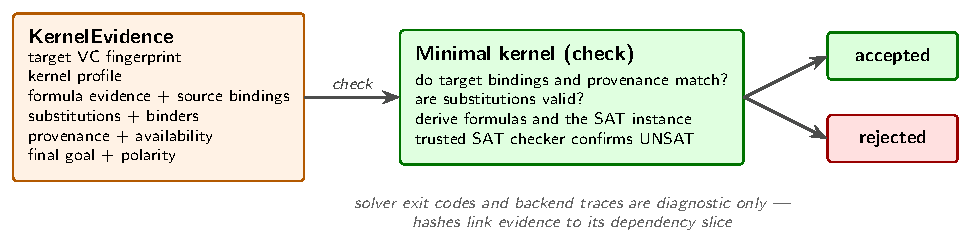
\includegraphics[width=\textwidth,height=0.52\textheight,keepaspectratio]{../2026-09-bialystok/figures/certificate_replay.pdf}
\end{center}
\begin{itemize}
\setlength{\itemsep}{1pt}
\setlength{\parsep}{0pt}
\setlength{\parskip}{0pt}
\item The evidence holds source formulas, explicit substitutions, provenance, and target and goal bindings. The kernel checks them, builds a deterministic SAT problem, and requires UNSAT from its trusted in-process SAT checker.
\item Backend proof traces, SMT proof objects, logs, and exit codes are for diagnosis only.
\end{itemize}
\note{
\smallskip
\textbf{Read aloud:}
\begin{itemize}
\setlength{\itemsep}{1pt}
\setlength{\parsep}{0pt}
\setlength{\parskip}{0pt}
\item The evidence holds source formulas, explicit substitutions, provenance, and target and goal bindings. The kernel checks them, builds a deterministic SAT problem, and requires UNSAT from its trusted in-process SAT checker.
\item Backend proof traces, SMT proof objects, logs, and exit codes are for diagnosis only.
\end{itemize}
\smallskip
\textbf{Optional notes and sources:}
\begin{itemize}
\setlength{\itemsep}{1pt}
\setlength{\parsep}{0pt}
\setlength{\parskip}{0pt}
\item Source: \texttt{doc/design/architecture/en/08.reasoning\_boundary.md}, \texttt{15.kernel\_certificate\_format.md}.
\end{itemize}
}
\end{frame}

\section{Backup 6. The Core ATP Path}
\begin{frame}[fragile,t]{Backup 6. The Core ATP Path}
\begin{center}
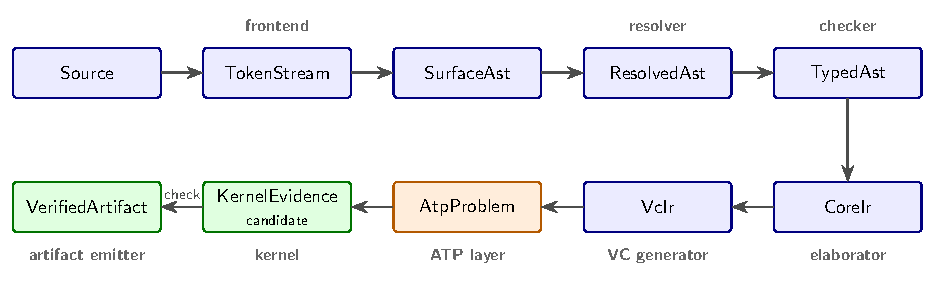
\includegraphics[width=\textwidth,height=0.52\textheight,keepaspectratio]{../2026-09-bialystok/figures/pipeline.pdf}
\end{center}
\begin{itemize}
\setlength{\itemsep}{1pt}
\setlength{\parsep}{0pt}
\setlength{\parskip}{0pt}
\item Only obligations that are still open after deterministic discharge go to ATPs. The earlier discharge also needs replayable evidence.
\item Each boundary states who owns a fact, which artifact records it, and what must be checked again after a change.
\end{itemize}
\note{
\smallskip
\textbf{Read aloud:}
\begin{itemize}
\setlength{\itemsep}{1pt}
\setlength{\parsep}{0pt}
\setlength{\parskip}{0pt}
\item Only obligations that are still open after deterministic discharge go to ATPs. The earlier discharge also needs replayable evidence.
\item Each boundary states who owns a fact, which artifact records it, and what must be checked again after a change.
\end{itemize}
\smallskip
\textbf{Optional notes and sources:}
\begin{itemize}
\setlength{\itemsep}{1pt}
\setlength{\parsep}{0pt}
\setlength{\parskip}{0pt}
\item Source: \texttt{doc/design/architecture/en/00.pipeline\_overview.md}; Bialystok deck, Part 10.
\end{itemize}
}
\end{frame}

\section{Backup 7. Incremental Verification}
\begin{frame}[fragile,t]{Backup 7. Incremental Verification}
\begin{center}
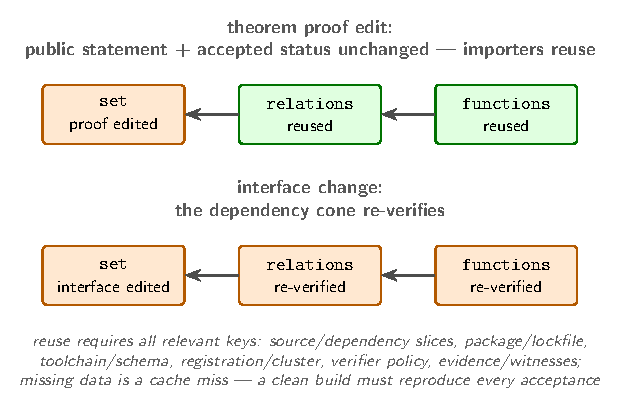
\includegraphics[width=\textwidth,height=0.52\textheight,keepaspectratio]{../2026-09-bialystok/figures/fingerprint_graph.pdf}
\end{center}
\begin{itemize}
\setlength{\itemsep}{1pt}
\setlength{\parsep}{0pt}
\setlength{\parskip}{0pt}
\item A proof-body edit does not rebuild importers when the exported statement and the accepted status stay the same. An interface change re-verifies the dependency cone.
\item All relevant cache keys must match; missing data is a cache miss. Cache reuse is never proof authority: a clean build must reproduce every acceptance.
\end{itemize}
\note{
\smallskip
\textbf{Read aloud:}
\begin{itemize}
\setlength{\itemsep}{1pt}
\setlength{\parsep}{0pt}
\setlength{\parskip}{0pt}
\item A proof-body edit does not rebuild importers when the exported statement and the accepted status stay the same. An interface change re-verifies the dependency cone.
\item All relevant cache keys must match; missing data is a cache miss. Cache reuse is never proof authority: a clean build must reproduce every acceptance.
\end{itemize}
\smallskip
\textbf{Optional notes and sources:}
\begin{itemize}
\setlength{\itemsep}{1pt}
\setlength{\parsep}{0pt}
\setlength{\parskip}{0pt}
\item Source: \texttt{doc/design/architecture/en/11.artifact\_and\_incremental\_build.md}, \texttt{18.dependency\_fingerprint.md}; Bialystok deck, Story 5.
\end{itemize}
}
\end{frame}

\section{Backup 8. Package Manifest}
\begin{frame}[fragile,t]{Backup 8. Package Manifest}
\smallskip
\textbf{Mizar Evo}~\badgeSpec
\begin{lstlisting}[language={toml},basicstyle=\ttfamily\footnotesize]
[package]
name    = "algebra"
version = "2.3.1"
edition = "2025"

[dependencies]
mml_core = "^1.0"
topology = { version = "^0.9", features = ["metric"] }
\end{lstlisting}
\begin{itemize}
\setlength{\itemsep}{1pt}
\setlength{\parsep}{0pt}
\setlength{\parskip}{0pt}
\item Reproducible builds need fixed source, lockfile, toolchain, and verifier settings, including deterministic ATP evidence.
\item Versioned reuse replaces manual copying between article sets; an aggregate module can export a whole topic through one import.
\end{itemize}
Source: \texttt{doc/spec/en/23.package\_management\_and\_build\_system.md}; Bialystok deck, Story 1.

\note{
\smallskip
\textbf{Read aloud:}
\begin{itemize}
\setlength{\itemsep}{1pt}
\setlength{\parsep}{0pt}
\setlength{\parskip}{0pt}
\item Reproducible builds need fixed source, lockfile, toolchain, and verifier settings, including deterministic ATP evidence.
\item Versioned reuse replaces manual copying between article sets; an aggregate module can export a whole topic through one import.
\end{itemize}
\smallskip
\textbf{Optional notes and sources:}
\begin{itemize}
\setlength{\itemsep}{1pt}
\setlength{\parsep}{0pt}
\setlength{\parskip}{0pt}
\item Source: \texttt{doc/spec/en/23.package\_management\_and\_build\_system.md}; Bialystok deck, Story 1.
\end{itemize}
}
\end{frame}

\section{Backup 9. Forty-Five-Minute Additions}
\begin{frame}[fragile,t]{Backup 9. Forty-Five-Minute Additions}
\smallskip
\textbf{Add selected examples where they fit in the story:}
\begin{enumerate}
\setlength{\itemsep}{1pt}
\setlength{\parsep}{0pt}
\setlength{\parskip}{0pt}
\item HOL-to-FOL function encoding worked through on one goal (\texttt{app}, partial application, lambda lifting).
\item Mizar function representation: \texttt{Function of X,Y}, \texttt{f.x}, soft type as a set-theoretic object.
\item Template: \texttt{PermProduct[T]} with additive and multiplicative views (Backup 4).
\item Algorithm: Euclidean GCD plus \texttt{by computation} and the promotion to a functor.
\item Structures and views: \texttt{AddMagma}, \texttt{MulMagma}, \texttt{Magma} (Bialystok Story 2).
\item Modern infrastructure: \texttt{mizar.pkg}, namespaces, the fingerprint graph (Backups 7-8).
\item Checking: evidence instantiation and the SAT check (Frame 6.3; details in Backup 5).
\end{enumerate}
\note{
\smallskip
\textbf{Read aloud:}
\begin{itemize}
\setlength{\itemsep}{1pt}
\setlength{\parsep}{0pt}
\setlength{\parskip}{0pt}
\item HOL-to-FOL function encoding worked through on one goal (\texttt{app}, partial application, lambda lifting).
\item Mizar function representation: \texttt{Function of X,Y}, \texttt{f.x}, soft type as a set-theoretic object.
\item Template: \texttt{PermProduct[T]} with additive and multiplicative views (Backup 4).
\item Algorithm: Euclidean GCD plus \texttt{by computation} and the promotion to a functor.
\item Structures and views: \texttt{AddMagma}, \texttt{MulMagma}, \texttt{Magma} (Bialystok Story 2).
\item Modern infrastructure: \texttt{mizar.pkg}, namespaces, the fingerprint graph (Backups 7-8).
\item Checking: evidence instantiation and the SAT check (Frame 6.3; details in Backup 5).
\end{itemize}
}
\end{frame}

\section{Backup 10. Sources And Attribution}
\begin{frame}[fragile,t]{Backup 10. Sources And Attribution}
\smallskip
\textbf{Exact MML excerpts used in this talk:}
\begin{scriptsize}
\setlength{\tabcolsep}{3pt}
\renewcommand{\arraystretch}{1.15}
\begin{tabularx}{\textwidth}{>{\raggedright\arraybackslash}X>{\raggedright\arraybackslash}X>{\raggedright\arraybackslash}X>{\raggedright\arraybackslash}X}
\toprule
\textbf{Purpose} & \textbf{Source} & \textbf{Lines} & \textbf{Used in} \\
\midrule
Function application \texttt{f.x} & \texttt{funct\_1.miz} & 138-140 & Frame 1.2 \\
\texttt{Function of X,Y} as a soft type & \texttt{funct\_2.miz} & 87-90 & Frame 1.2 \\
\bottomrule
\end{tabularx}
\end{scriptsize}

\smallskip
\textbf{Source URLs:}
\begin{itemize}
\setlength{\itemsep}{1pt}
\setlength{\parsep}{0pt}
\setlength{\parskip}{0pt}
\item \texttt{FUNCT\_1}: \url{https://mizar.uwb.edu.pl/version/current/mml/funct\_1.miz}
\item \texttt{FUNCT\_2}: \url{https://mizar.uwb.edu.pl/version/current/mml/funct\_2.miz}
\end{itemize}
\smallskip
\textbf{Attribution note:}
\begin{itemize}
\setlength{\itemsep}{1pt}
\setlength{\parsep}{0pt}
\setlength{\parskip}{0pt}
\item MML plain-text files state GPL-3.0-or-later / CC-BY-SA-3.0-or-later terms; keep article attribution, URLs, and line numbers in speaker notes.
\item Benchmark figures: see Backups 1-2 and \texttt{references.bib}. Verify bibliographic metadata against publishers before the final deck.
\end{itemize}
\note{
\smallskip
\textbf{Read aloud:}
\begin{itemize}
\setlength{\itemsep}{1pt}
\setlength{\parsep}{0pt}
\setlength{\parskip}{0pt}
\item \texttt{FUNCT\_1}: \url{https://mizar.uwb.edu.pl/version/current/mml/funct\_1.miz}
\item \texttt{FUNCT\_2}: \url{https://mizar.uwb.edu.pl/version/current/mml/funct\_2.miz}
\item MML plain-text files state GPL-3.0-or-later / CC-BY-SA-3.0-or-later terms; keep article attribution, URLs, and line numbers in speaker notes.
\item Benchmark figures: see Backups 1-2 and \texttt{references.bib}. Verify bibliographic metadata against publishers before the final deck.
\end{itemize}
}
\end{frame}

\section{Backup 11. Comparing Evaluation Conditions}
\begin{frame}[fragile,t]{Backup 11. Comparing Evaluation Conditions}
\begin{scriptsize}
\setlength{\tabcolsep}{3pt}
\renewcommand{\arraystretch}{1.15}
\begin{tabularx}{\textwidth}{>{\raggedright\arraybackslash}X>{\raggedright\arraybackslash}X>{\raggedright\arraybackslash}X}
\toprule
\textbf{} & \textbf{MizAR 60 (ITP 2023)} & \textbf{Sledgehammer / AFP (ITP 2022)} \\
\midrule
success & 58.4\% (1,690 / 2,896) & 68.8\% (3,440 / 5,000) \\
counts & MML 1147: 2,896 holdout theorems/lemmas (57,897 total) & 5,000 local goals; 50 AFP entries \\
premises & learned selection from the whole library & MePo; base 512 facts, varied by configuration \\
budget & portfolio: 420 CPU s & 16 greedy configurations, 30 CPU s each: 480 CPU s \\
status & ATP proof found (hammering) & external proof found; no Isabelle reconstruction \\
\bottomrule
\end{tabularx}
\end{scriptsize}

\begin{itemize}
\setlength{\itemsep}{1pt}
\setlength{\parsep}{0pt}
\setlength{\parskip}{0pt}
\item \textcolor{blue!55!black}{\textbf{Different units, premises, budgets, and configurations; the rates do not rank the designs.}}
\end{itemize}
\note{
\smallskip
\textbf{Read aloud:}
\begin{itemize}
\setlength{\itemsep}{1pt}
\setlength{\parsep}{0pt}
\setlength{\parskip}{0pt}
\item \textcolor{blue!55!black}{\textbf{Different units, premises, budgets, and configurations; the rates do not rank the designs.}}
\end{itemize}
\smallskip
\textbf{Optional notes and sources:}
\begin{itemize}
\setlength{\itemsep}{1pt}
\setlength{\parsep}{0pt}
\setlength{\parskip}{0pt}
\item A "hammer" is a tool that sends a goal to automatic provers. "Premises" are the facts the prover may use.
\item Source: Jakubův et al. 2023, sections 6.2, 6.5; Desharnais et al. 2022, sections 5, 5.6, Table 10. The greedy configurations were selected using the evaluation set itself.
\item Publication dates differ from experiment dates. MizAR's main experiments ran in 2020-2021; the AFP study uses Isabelle from January 2022 and AFP from December 2021.
\item MizAR's 75\% figure uses premises chosen from the library by a human or a machine. Keep it for questions.
\end{itemize}
}
\end{frame}

\section{Backup 12. What Each Number Counts}
\begin{frame}[fragile,t]{Backup 12. What Each Number Counts}
\begin{center}
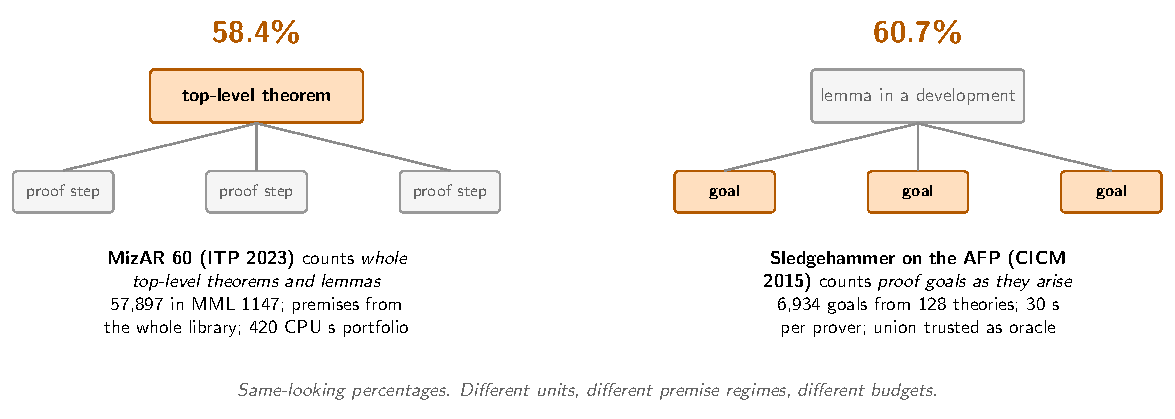
\includegraphics[width=\textwidth,height=0.5\textheight,keepaspectratio]{figures/evaluation_units.pdf}
\end{center}
\begin{itemize}
\setlength{\itemsep}{1pt}
\setlength{\parsep}{0pt}
\setlength{\parskip}{0pt}
\item \textcolor{blue!55!black}{\textbf{MizAR asks: can the machine prove this whole theorem from the library, with no help from the author?}}
\item \textcolor{blue!55!black}{\textbf{The AFP study asks: can the machine close this goal where it appears, often inside a proof that a person has already written?}}
\item Both are fair questions. They are not the same question.
\end{itemize}
\note{
\smallskip
\textbf{Read aloud:}
\begin{itemize}
\setlength{\itemsep}{1pt}
\setlength{\parsep}{0pt}
\setlength{\parskip}{0pt}
\item \textcolor{blue!55!black}{\textbf{MizAR asks: can the machine prove this whole theorem from the library, with no help from the author?}}
\item \textcolor{blue!55!black}{\textbf{The AFP study asks: can the machine close this goal where it appears, often inside a proof that a person has already written?}}
\item Both are fair questions. They are not the same question.
\end{itemize}
}
\end{frame}

\section{Backup 13. Two Paths To A First-Order Prover}
\begin{frame}[fragile,t]{Backup 13. Two Paths To A First-Order Prover}
\begin{center}
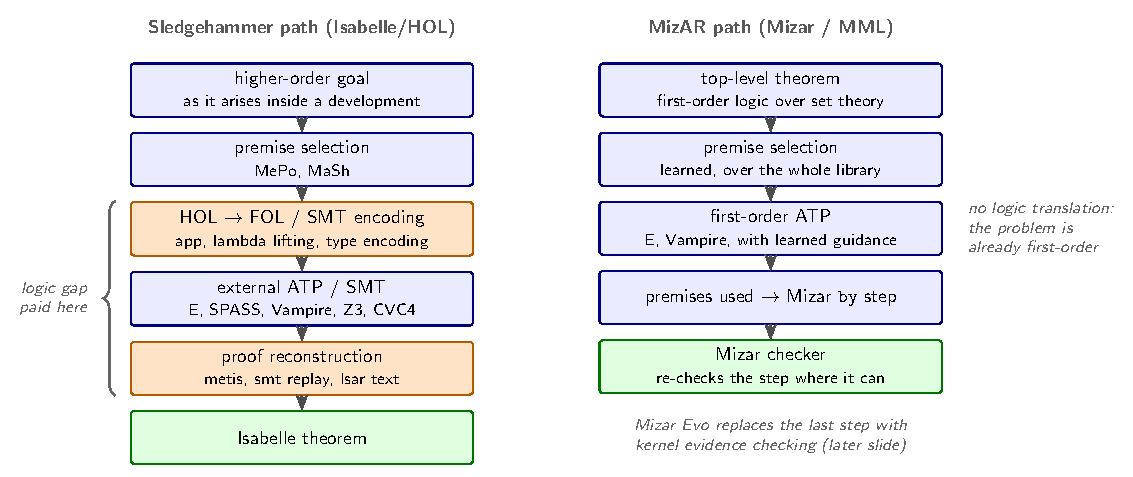
\includegraphics[width=\textwidth,height=0.58\textheight,keepaspectratio]{figures/two_paths.pdf}
\end{center}
\begin{itemize}
\setlength{\itemsep}{1pt}
\setlength{\parsep}{0pt}
\setlength{\parskip}{0pt}
\item \textcolor{blue!55!black}{\textbf{In Sledgehammer's first-order and SMT path, a higher-order goal is translated, and the proof is rebuilt inside Isabelle.}}
\item \textcolor{blue!55!black}{\textbf{MizAR gives the prover a problem that is already first-order. The generated problem is first-order.}}
\end{itemize}
\note{
\smallskip
\textbf{Read aloud:}
\begin{itemize}
\setlength{\itemsep}{1pt}
\setlength{\parsep}{0pt}
\setlength{\parskip}{0pt}
\item \textcolor{blue!55!black}{\textbf{In Sledgehammer's first-order and SMT path, a higher-order goal is translated, and the proof is rebuilt inside Isabelle.}}
\item \textcolor{blue!55!black}{\textbf{MizAR gives the prover a problem that is already first-order. The generated problem is first-order.}}
\end{itemize}
\smallskip
\textbf{Optional notes and sources:}
\begin{itemize}
\setlength{\itemsep}{1pt}
\setlength{\parsep}{0pt}
\setlength{\parskip}{0pt}
\item Both paths describe existing systems (Blanchette, Kaliszyk, Paulson, Urban 2016; Jakubův et al. 2023). The orange boxes are the translation and reconstruction layers.
\item The figure shows the first-order and SMT path. The ITP 2022 evaluation also includes provers using native higher-order formats.
\item MizAR's headline percentages count ATP proofs. The Mizar checker re-checks the resulting \texttt{by} step when the inference is within its strength.
\end{itemize}
}
\end{frame}

\section{Backup 14. Functions In Higher-Order Logic}
\begin{frame}[fragile,t]{Backup 14. Functions In Higher-Order Logic}
\smallskip
\textbf{Schematic HOL statement}~\badgeSketch~{\footnotesize(Isabelle/HOL-style notation)}
\begin{lstlisting}[language={},basicstyle=\ttfamily\small]
f :: 'a => 'b        x :: 'a

P (f x)
\end{lstlisting}
\begin{itemize}
\setlength{\itemsep}{1pt}
\setlength{\parsep}{0pt}
\setlength{\parskip}{0pt}
\item \textcolor{blue!55!black}{\textbf{In HOL, function types and function application are part of the logic itself.}}
\item Functions as arguments, functions that return functions, partial application, lambda: all can be written directly.
\item \textcolor{blue!55!black}{\textbf{This is very convenient for the person who writes mathematics.}}
\item \textcolor{blue!55!black}{\textbf{But E and Vampire are first-order provers. The higher-order structure must be encoded before they can see it.}}
\end{itemize}
\note{
\smallskip
\textbf{Read aloud:}
\begin{itemize}
\setlength{\itemsep}{1pt}
\setlength{\parsep}{0pt}
\setlength{\parskip}{0pt}
\item Schematic HOL statement.
\item \textcolor{blue!55!black}{\textbf{In HOL, function types and function application are part of the logic itself.}}
\item Functions as arguments, functions that return functions, partial application, lambda: all can be written directly.
\item \textcolor{blue!55!black}{\textbf{This is very convenient for the person who writes mathematics.}}
\item \textcolor{blue!55!black}{\textbf{But E and Vampire are first-order provers. The higher-order structure must be encoded before they can see it.}}
\end{itemize}
}
\end{frame}

\section{Backup 15. HOL Encoding And Reconstruction}
\begin{frame}[fragile,t]{Backup 15. HOL Encoding And Reconstruction}
\smallskip
\textbf{Encoding steps, schematic}~\badgeSketch
\begin{lstlisting}[language={},basicstyle=\ttfamily\footnotesize]
F X                   ->  app(F, X)
(%x. t) ...           ->  fresh constant + defining axioms   (lambda lifting)
polymorphic types     ->  type guards or type tags
Boolean-valued terms  ->  extra encoding
\end{lstlisting}
\begin{itemize}
\setlength{\itemsep}{1pt}
\setlength{\parsep}{0pt}
\setlength{\parskip}{0pt}
\item \textcolor{blue!55!black}{\textbf{Applying a variable function becomes an explicit \texttt{app} symbol. Lambdas are lifted out or turned into combinators. Types become guards or tags.}}
\item \textcolor{blue!55!black}{\textbf{After the prover succeeds, the proof must come back into Isabelle: a \texttt{metis} call, an \texttt{smt} replay, or generated Isar text. This step is called reconstruction.}}
\item These mechanisms connect HOL goals to first-order provers.
\item This describes the connection, not a measured performance ranking.
\end{itemize}
\note{
\smallskip
\textbf{Read aloud:}
\begin{itemize}
\setlength{\itemsep}{1pt}
\setlength{\parsep}{0pt}
\setlength{\parskip}{0pt}
\item Encoding steps, schematic.
\item \textcolor{blue!55!black}{\textbf{Applying a variable function becomes an explicit \texttt{app} symbol. Lambdas are lifted out or turned into combinators. Types become guards or tags.}}
\item \textcolor{blue!55!black}{\textbf{After the prover succeeds, the proof must come back into Isabelle: a \texttt{metis} call, an \texttt{smt} replay, or generated Isar text. This step is called reconstruction.}}
\item These mechanisms connect HOL goals to first-order provers.
\item This describes the connection, not a measured performance ranking.
\end{itemize}
\smallskip
\textbf{Optional notes and sources:}
\begin{itemize}
\setlength{\itemsep}{1pt}
\setlength{\parsep}{0pt}
\setlength{\parskip}{0pt}
\item Source: Meng and Paulson 2008 (translating higher-order clauses to first-order clauses); Blanchette, Böhme, Popescu, Smallbone 2016 (type encodings); Blanchette, Kaliszyk, Paulson, Urban 2016 (survey); Schurr, Fleury, Desharnais 2021 (reconstruction).
\item The exact encodings that Sledgehammer uses depend on the prover and the options. This frame is schematic.
\end{itemize}
}
\end{frame}

\section{Backup 16. Where Complexity Lives}
\begin{frame}[fragile,t]{Backup 16. Where Complexity Lives}
\begin{center}
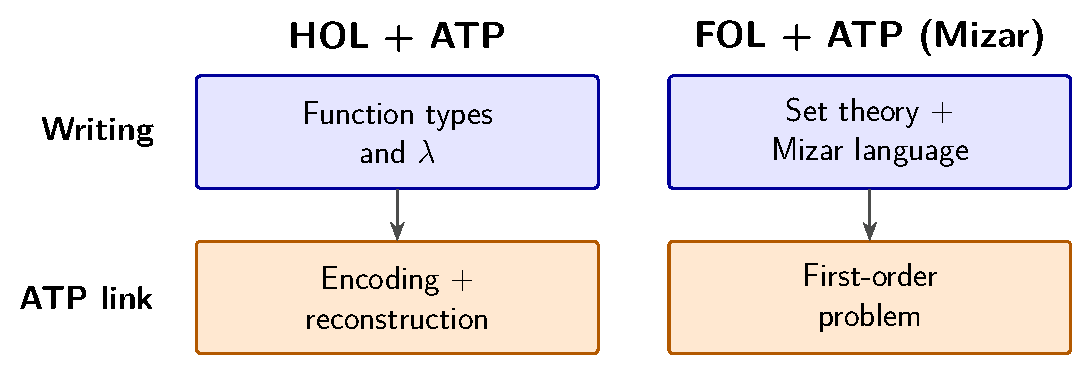
\includegraphics[width=\textwidth,height=0.54\textheight,keepaspectratio]{figures/where_you_pay.pdf}
\end{center}
\begin{itemize}
\setlength{\itemsep}{1pt}
\setlength{\parsep}{0pt}
\setlength{\parskip}{0pt}
\item \textcolor{blue!55!black}{\textbf{HOL encodes higher-order structures for ATPs. Mizar's language hides set-theoretic details.}}
\item \textcolor{blue!55!black}{\textbf{Mizar Evo keeps the first-order foundation and modernizes mathematical writing.}}
\end{itemize}
\note{
\smallskip
\textbf{Read aloud:}
\begin{itemize}
\setlength{\itemsep}{1pt}
\setlength{\parsep}{0pt}
\setlength{\parskip}{0pt}
\item \textcolor{blue!55!black}{\textbf{HOL encodes higher-order structures for ATPs. Mizar's language hides set-theoretic details.}}
\item \textcolor{blue!55!black}{\textbf{Mizar Evo keeps the first-order foundation and modernizes mathematical writing.}}
\end{itemize}
\smallskip
\textbf{Optional notes and sources:}
\begin{itemize}
\setlength{\itemsep}{1pt}
\setlength{\parsep}{0pt}
\setlength{\parskip}{0pt}
\item HOL and FOL put complexity in different layers. HOL has function types and lambdas in its logic; its first-order ATP path uses encoding and reconstruction.
\item Mizar's soft types, modes, attributes, registrations, and schemes hide details such as pairs and domains that appear in raw set-theoretic writing.
\end{itemize}
}
\end{frame}

\section{Backup 17. Design Trade-Offs}
\begin{frame}[fragile,t]{Backup 17. Design Trade-Offs}
\begin{scriptsize}
\setlength{\tabcolsep}{3pt}
\renewcommand{\arraystretch}{1.15}
\begin{tabularx}{\textwidth}{>{\raggedright\arraybackslash}X>{\raggedright\arraybackslash}X>{\raggedright\arraybackslash}X}
\toprule
\textbf{} & \textbf{HOL ITP + ATP} & \textbf{FOL ITP + ATP} \\
\midrule
writing & higher-order features, short text & long text if written raw \\
functions & basic higher-order objects & first-order set-theoretic objects \\
ATP connection & HOL-to-FOL / SMT encoding & generation of a first-order problem \\
reconstruction & reconstruction in Isabelle & rechecking Mizar steps where supported \\
the language must provide & HOL abstraction & abstraction that hides first-order details \\
\bottomrule
\end{tabularx}
\end{scriptsize}

\begin{itemize}
\setlength{\itemsep}{1pt}
\setlength{\parsep}{0pt}
\setlength{\parskip}{0pt}
\item This table compares representations and checking paths. It gives no measured performance advantage.
\end{itemize}
\note{
\smallskip
\textbf{Read aloud:}
\begin{itemize}
\setlength{\itemsep}{1pt}
\setlength{\parsep}{0pt}
\setlength{\parskip}{0pt}
\item This table compares representations and checking paths. It gives no measured performance advantage.
\end{itemize}
}
\end{frame}

\end{document}
